In the current context the word \textit{inference} simply means to uncover evidence of certain features or behaviors of an archetype to the point where it is valid to make an interpretation of what the main objective of the archetype is. As such, ParTI is really a method for \textit{providing evidence} rather than giving an ultimate answer.

Since archetypes in trait-space are optimal configurations of traits for performing specific objectives that are evolutionarily important, the problem of inferring what those objectives are can be solved in many ways. For very simple systems one could unobtrusively observe how organisms employ their traits and take special notice of behavioral differences between those that resemble archetypes\mcite{shoval2012evolutionary}. But for systems that can't be directly observed, other methods must be used. A relevant example is personalities of people and which behavioral strategies for performing evolutionarily important tasks they lead to. In this example traits are personality factors such as the Big Five (see Section \ref{subsubsec:dimensionsOfPersonality}) and the objective is the behavioral strategy that the personality is optimized to perform. Given the archetypes it would be to time-consuming and obtrusive to monitor people, who were similar to each archetype, in their natural habitat. Using qualitative interviewing might work better but would also be time consuming and possibly introduce qualitative research biases.

A better approach is to study the statistical properties of individuals who are similar to each archetype. Using \textit{extra data} such as demographic variables, response items from surveys and behavioral data, layers of information can be added such as to reveal what people similar to each archetype typically do for a living, whether they tend to be married or what age range they occupy. This approach is general. If the system were cancer cells and traits were gene expressions, extra data such as tissue type, cell cycle period and protein production level would provide evidence to aid inference of objectives for different cells\mcite{hart2015inferring}.

There are different methods for doing this. The simplest method is to correlate the feature value with distance from the archetype and then use the slope and correlation coefficient as measures of relatedness.
Another approach which provides a better visual image is to analyze the \textit{enrichment} of features near the archetypes. As illustrated in Figure \ref{fig:enrichmentExample} this method works by binning points according to their distance from the archetype and then taking the average of the feature in each bin to create a curve which shows whether the feature tends to be enriched or \textit{depleted} near the archetype. If the feature is categorical the method estimates the frequency of each category in every bin, such as to create separate histograms for the feature-categories. This method is applied widely in ParTI literature\mcite{korem2015geometry, szekely2015mass, tendler2015evolutionary, shoval2012evolutionary, hart2015inferring}.

\begin{figure}
	\centering
	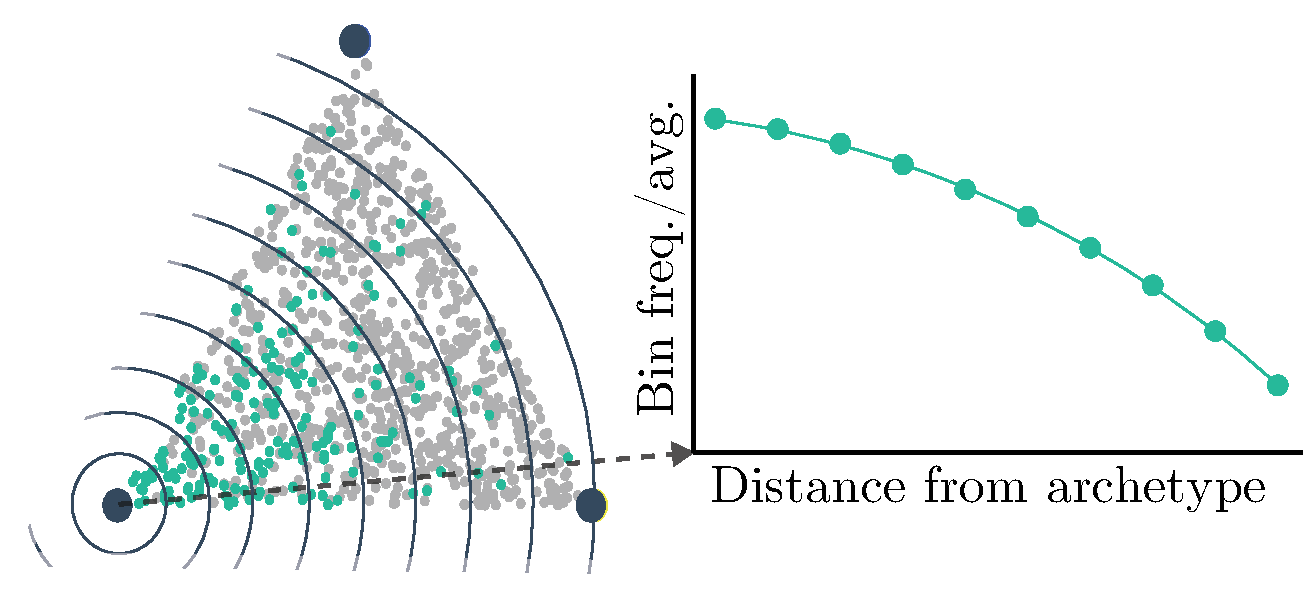
\includegraphics[width=0.7\textwidth]{figures/enrichmentExample}
	\caption{\label{fig:enrichmentExample} Enrichment of variables near archetypes are estimated across a number bins characterized by distance to the archetype. If the studied feature is continuous the }
\end{figure}